\section{Einleitung}\label{sec:Einleitung}
%

Der Transportsektor trägt in der EU mit einem Anteil von ca. 25\% signifikant zu der gesamten Treibhausgasemission (THG) bei. Um die Ziele der EU-Kommission zu erreichen, soll bis 2030 die Anzahl der Fahrzeuge mit konventionellem Antrieb halbiert werden. Bis 2050 soll auf Fahrzeuge mit Benzin- oder Diesel-Motoren komplett verzichtet werden.\\
Eines der Hindernisse für eine Marktdurchdringung der Fahrzeuge mit elektrochemischen Energiespeicher in Form von Lithium-Ionen-Batterien (LIB's) ist die begrenzte Reichweite dieser Fahrzeugklasse\footcite[Vgl.][S.136-146]{Ajanovic2020}.\\
Die Energiedichte von aktuellen LIB's\footcite[Vgl.][S. 11]{Hettesheimer2017} liegt nach Tabelle \ref{tab:Energiedichten} weit unter der von konventionellen Treibstoffen\footcite[Vgl.][]{BeloitEDU2021}. Da auch die Batterie-Aufladezeiten ein Vielfaches der Dauer einer Tankfüllung mit einem Flüssigtreibstoff beträgt, haben Verluste die durch Widerstand oder Abwärme entstehen, zusammen mit Leistung die für das Kühlen bzw. Aufheizen der Batterie aufgewendet werden muss, einen signifikant negativen Effekt auf die Reichweite und Effizienz der Fahrzeuge.\\

\begin{table}[H]
	\caption{Vergleich der Energiedichten von Energieträgern in Fahrzeugen}
	\label{tab:Energiedichten}
	\vspace{0.2cm}	
	\begin{tabularx}{\textwidth}{ |X|X|X|  }
		\toprule[1.5pt]
		\textbf{Typ} & \textbf{Wert} & \textbf{Einheit} \\
		\hline\hline
		Lithium-Ionen-Batterie: & 430 - 800 & Wh/l \\
		\hline
		Benzin: & 9700 & Wh/l \\
		\hline
		Diesel: & 10700 & Wh/l \\
		\bottomrule[1.5pt]
	\end{tabularx}		
\end{table}

















%
%%\cref{fig:Blume} zeigt ein Beispiel für eine Abbildung.
%\begin{figure}[H]
%	\flushleft
%	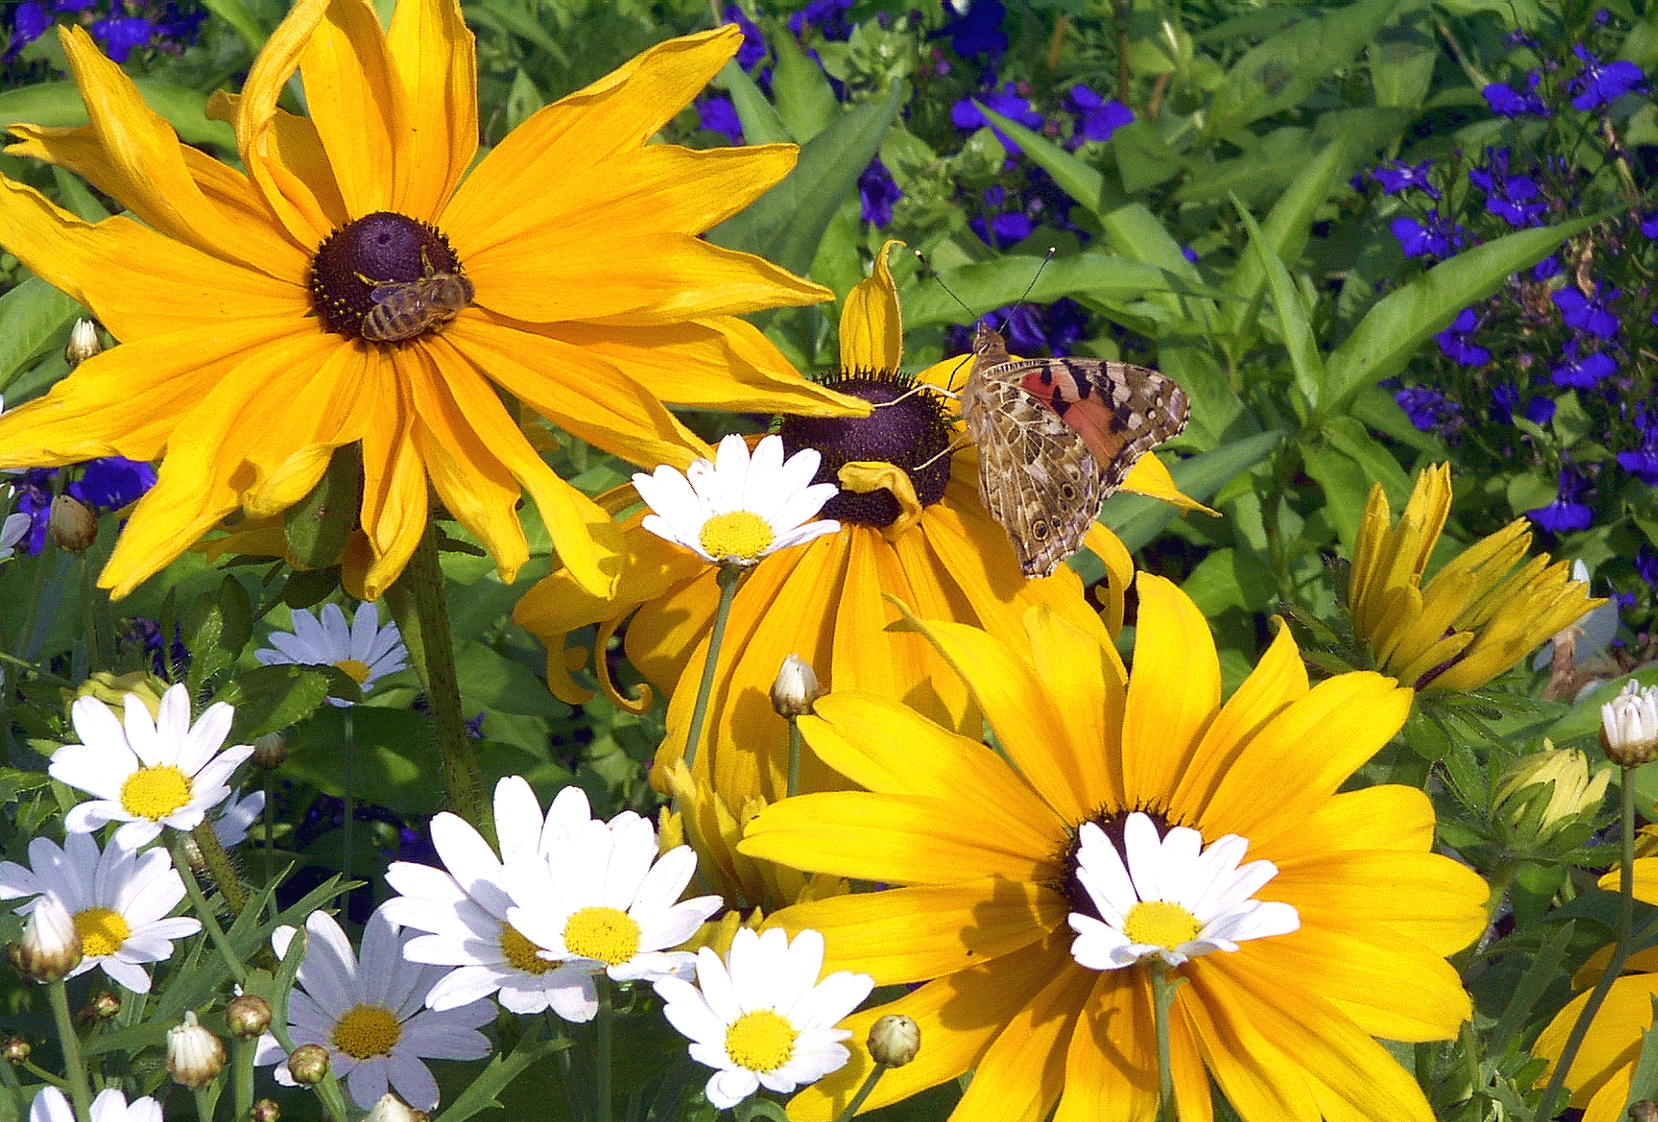
\includegraphics[scale=0.2]{figs/Blume.jpeg}
%	\caption{dies ist eine schöne Blume}
%	\label{fig:Blume} 
%\end{figure}
%\noindent
%\cref{eq:Formel} zeigt ein Beispiel für eine Formel.
%\begin{align}\label{eq:Formel}
%	I = \int_{t_0}^{t_0+n \cdot h} f(t) \hspace{0.1cm} dt
%\end{align}
%\noindent
%\cref{tab:Tabelle} zeig ein Beispiel für eine Tabelle
%\begin{table}[H]
%	\flushleft
%	\caption{Tabelle}
%	\label{tab:Tabelle} 
%	\vspace{0.2cm}
%	\begin{tabularx}{\textwidth}{p{3.5cm}XXXXXXX}
%		\toprule[1.5pt]
%		ABC: & 1 & 2 & 3 \\
%		\midrule[1.0pt]
%		DEF: & 4 & 5 & 6 \\
%		\bottomrule[1.5pt]	
%	\end{tabularx}
%\end{table}
%\noindent
%Zitiert wird mit "footcite". Das sieht dann so %\footcite[Vgl.][S. 456]{PeterPan2017} oder so\footcite[Vgl.][S. 123]{DEF2014} aus.
%%
%\subsection{Unterkapitel 1}\label{subsec:Unterkapitel1}
%%
%%
%\subsection{Unterkapitel 2}\label{subsec:Unterkapitel2}
%%
%\subsubsection{Unterkapitel 2.1}\label{subsec:Unterkapitel2.1}
%%
%
%


